%%%%%%%%%%%%%%% Pacotes utilizados
\documentclass[a4paper, 12pt]{article}
\usepackage[T1]{fontenc}
\usepackage[brazil]{babel}
\usepackage[utf8]{inputenc}
\usepackage{verbatim}
\usepackage[normalem]{ulem} %para 
\usepackage{indentfirst}
\usepackage{setspace}
\usepackage{float}
\usepackage{fancyhdr}
\usepackage{graphicx}


%%%%%%%%%%%%%%% Configurações
\setlength{\textwidth}{16cm}
\setlength{\textheight}{23cm}
\setlength{\evensidemargin}{-1cm} 
\setlength{\oddsidemargin}{0.5cm}
\setlength{\topmargin}{0cm}
\pagestyle{fancy}
\fancyhf{}
\lhead{\textbf{Nome:} Jhonatan Guilherme de Oliveira Cunha}
\rhead{\textbf{RA:} 2135590}
\cfoot{\thepage}
\hoffset= -0.4cm
\voffset=-0.9cm


%%%%%%%%%%%%% Início do documento
\begin{document}
	
	\hspace{5cm}
	
	\begin{large}
		\begin{center}
			\textbf{UNIVERSIDADE TECNOLÓGICA FEDERAL DO PARANÁ}\newline
			\textbf{CAMPUS CAMPO MOURÃO}
		\end{center}
	\end{large}
	
	\vspace{0.5cm}
	
	\begin{center}
		\textbf{BANDO DE DADOS 1 - LISTA MODELO ENTIDADE RELACIONAMENTO}
	\end{center}

	\vspace{0.5cm}
	

	
	
	\begin{enumerate}
		
		\item \textbf{Pizzaria:} Uma pizzaria de delivery apresenta um cardápio composto por diversos tipos de pizza, cujos
		dados são: número do item, nome da pizza, lista de ingredientes e preços das pizzas pequena,
		média e grande, como por exemplo: (12, francesa, (queijo, presunto, champignon, aspargo),
		10.00, 15.00, 18.00). Na pizzaria trabalham funcionários que emitem pedidos de pizzas. Cada
		pedido possui um número e uma data de emissão, além do nome, telefone e endereço do
		cliente que solicitou o pedido. Além disso, um pedido, que é emitido por apenas um funcionário,
		é composto por vários itens: cada item possui um número e se refere a uma determinada
		pizza do cardápio, em um determinado tamanho (pequena, média ou grande) e em uma certa
		quantidade. Dos funcionários entregadores (ou seja, responsáveis pela entrega de um ou mais
		pedidos), deve-se saber o número do telefone celular para um eventual contato durante uma
		entrega. Uma entrega destina-se a um bairro, e para cada bairro existe um tempo máximo de
		espera para a entrega de um pedido. Defina outros atributos que julgar relevante.
		
		\begin{figure}[H]
			\centering
			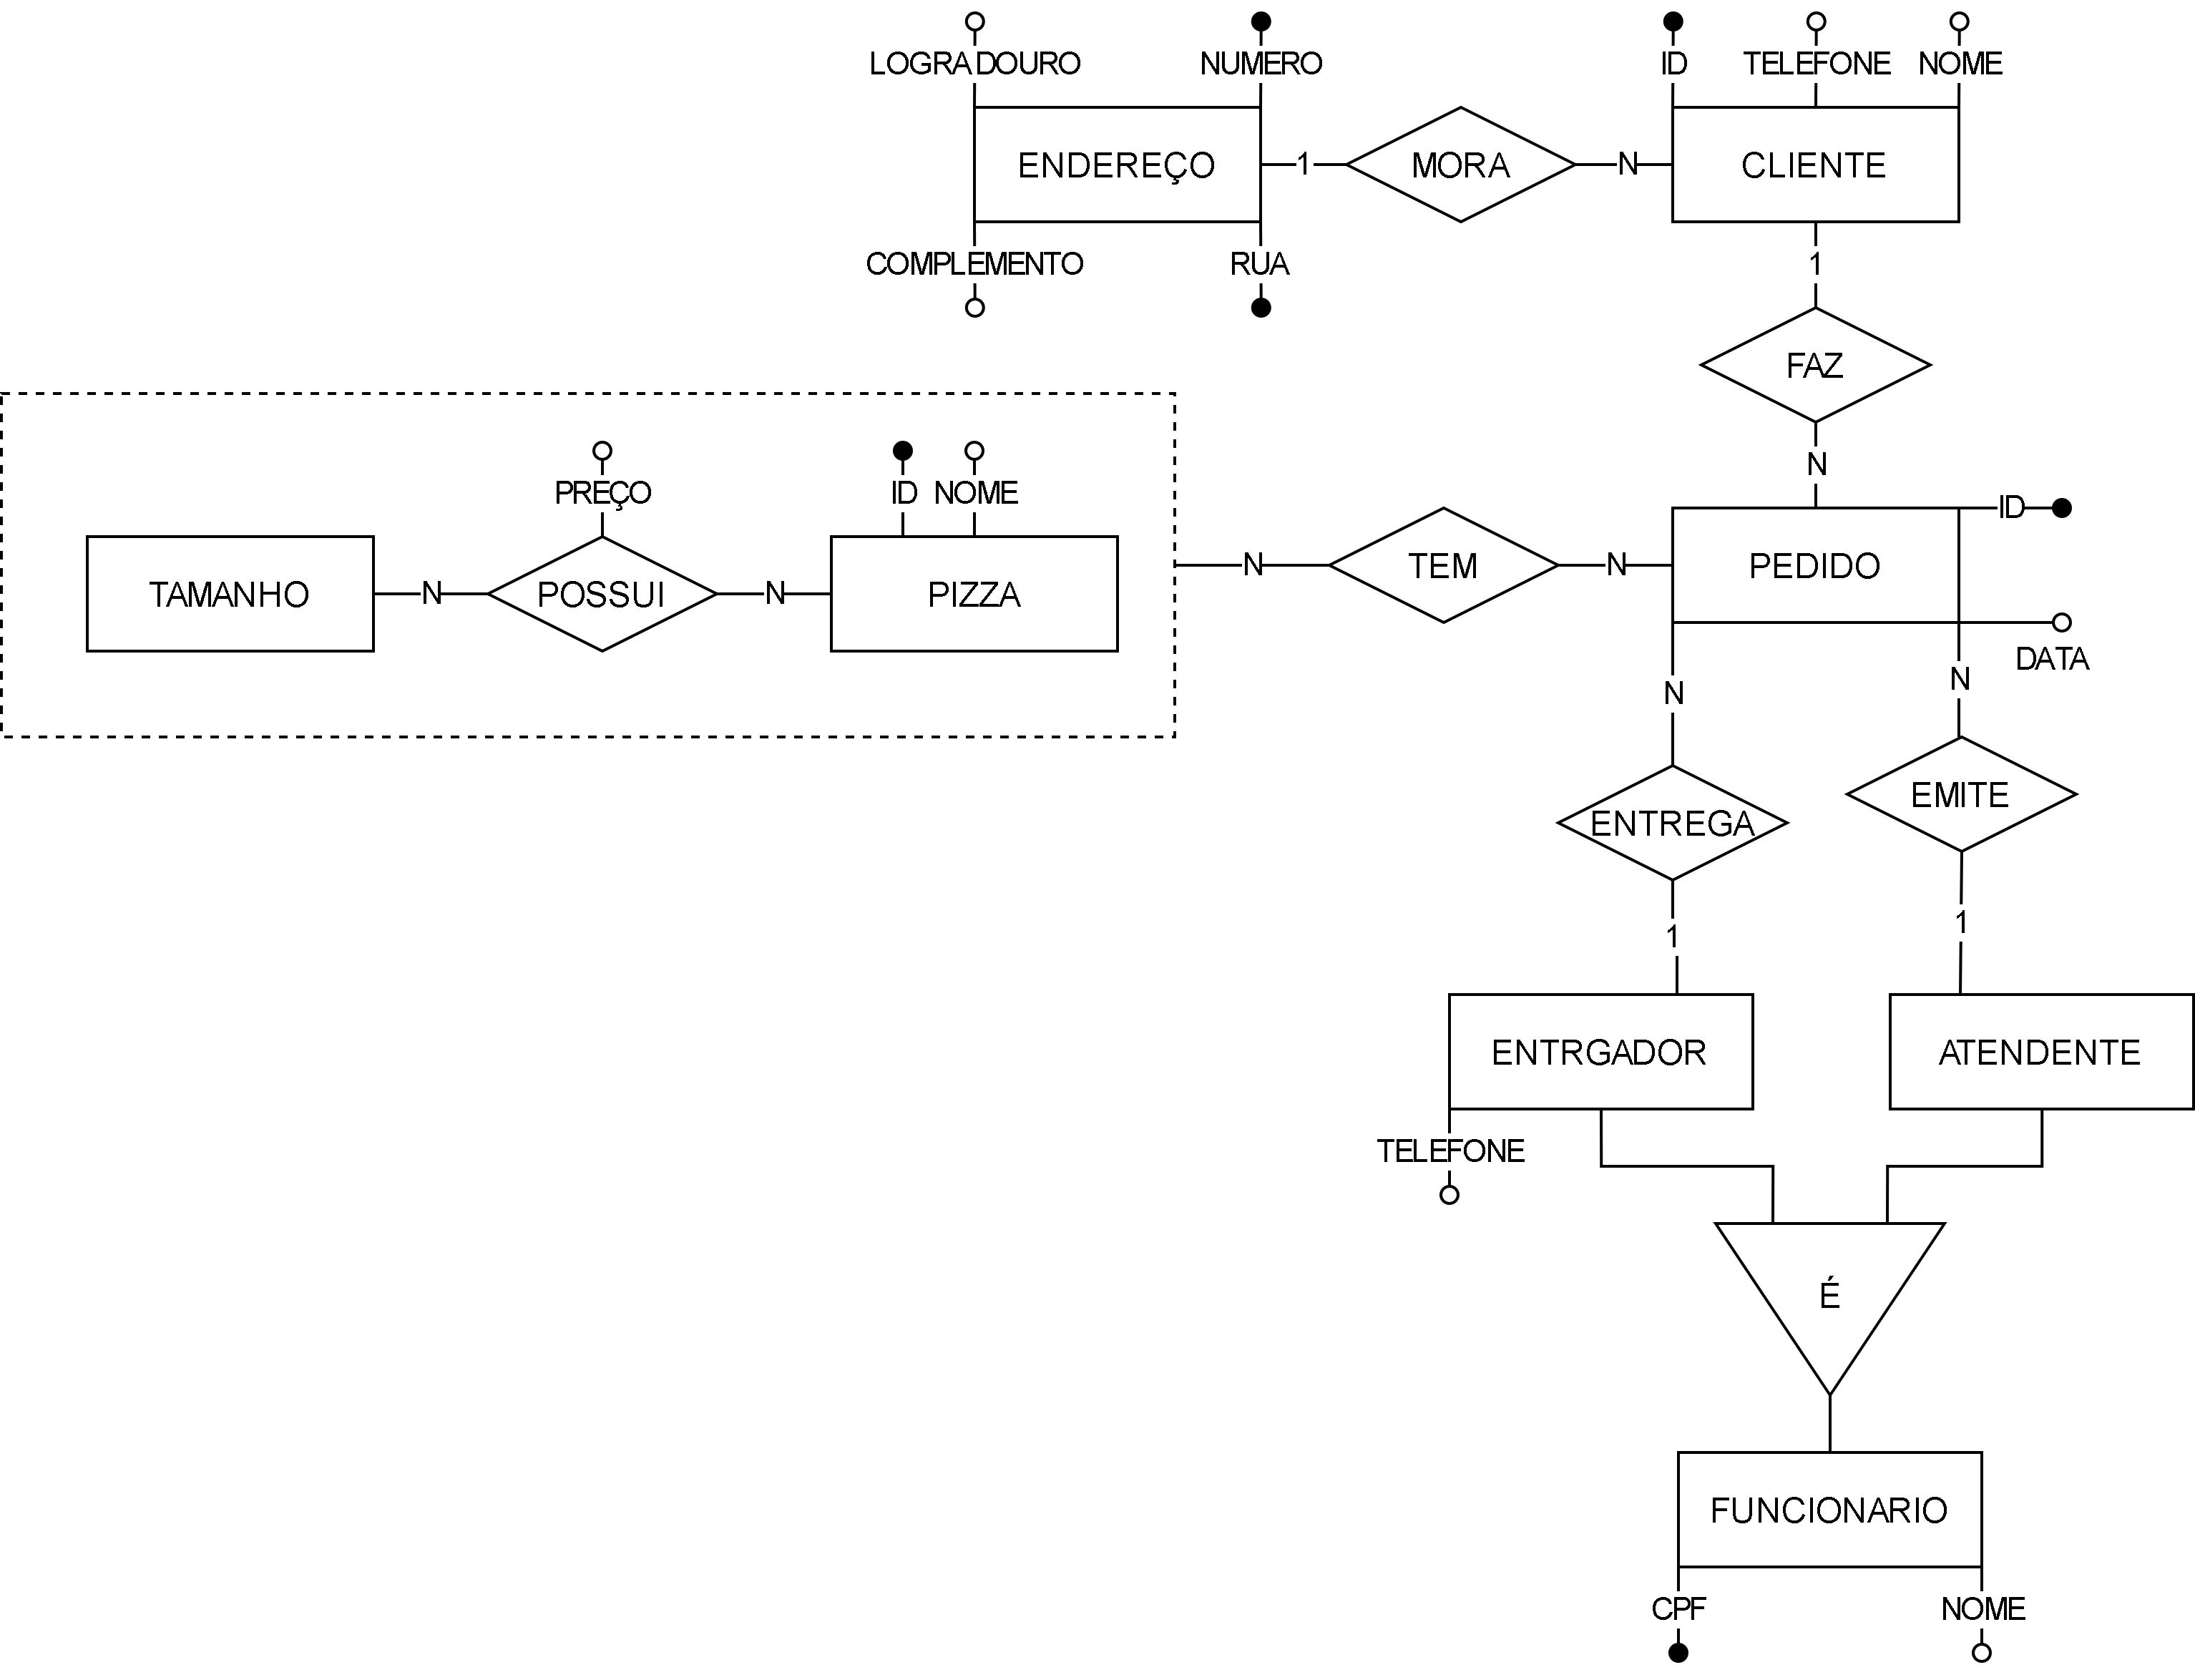
\includegraphics[width=0.85\textwidth]{LISTA 01 - EX 1 RESOLUÇÃO.png}
		\end{figure}
		\newpage
		
		\onehalfspacing
		\item \textbf{Clinica Médica:} Em uma clínica trabalham médicos de diversas especialidades. Cada médico é identificado
		pelo seu CRM, possui um nome e recebe um salário na clínica. Um médico pode ter formação em diversas especialidades (ortopedia, traumatologia, etc), mas só exerce uma delas
		na clínica. Para todo paciente internado na clínica são cadastrados alguns dados pessoais:
		nome, RG, CPF, endereço, telefone(s) para contato e data do nascimento. Um paciente tem
		sempre um determinado médico como responsável (com um horário de visita diário predeterminado), porém vários outros médicos podem participar do seu tratamento. Pacientes estão
		sempre internados em quartos individuais, que são identificados por um número e ficam em
		um andar da clínica. 
		
		\begin{figure}[H]
			\centering
			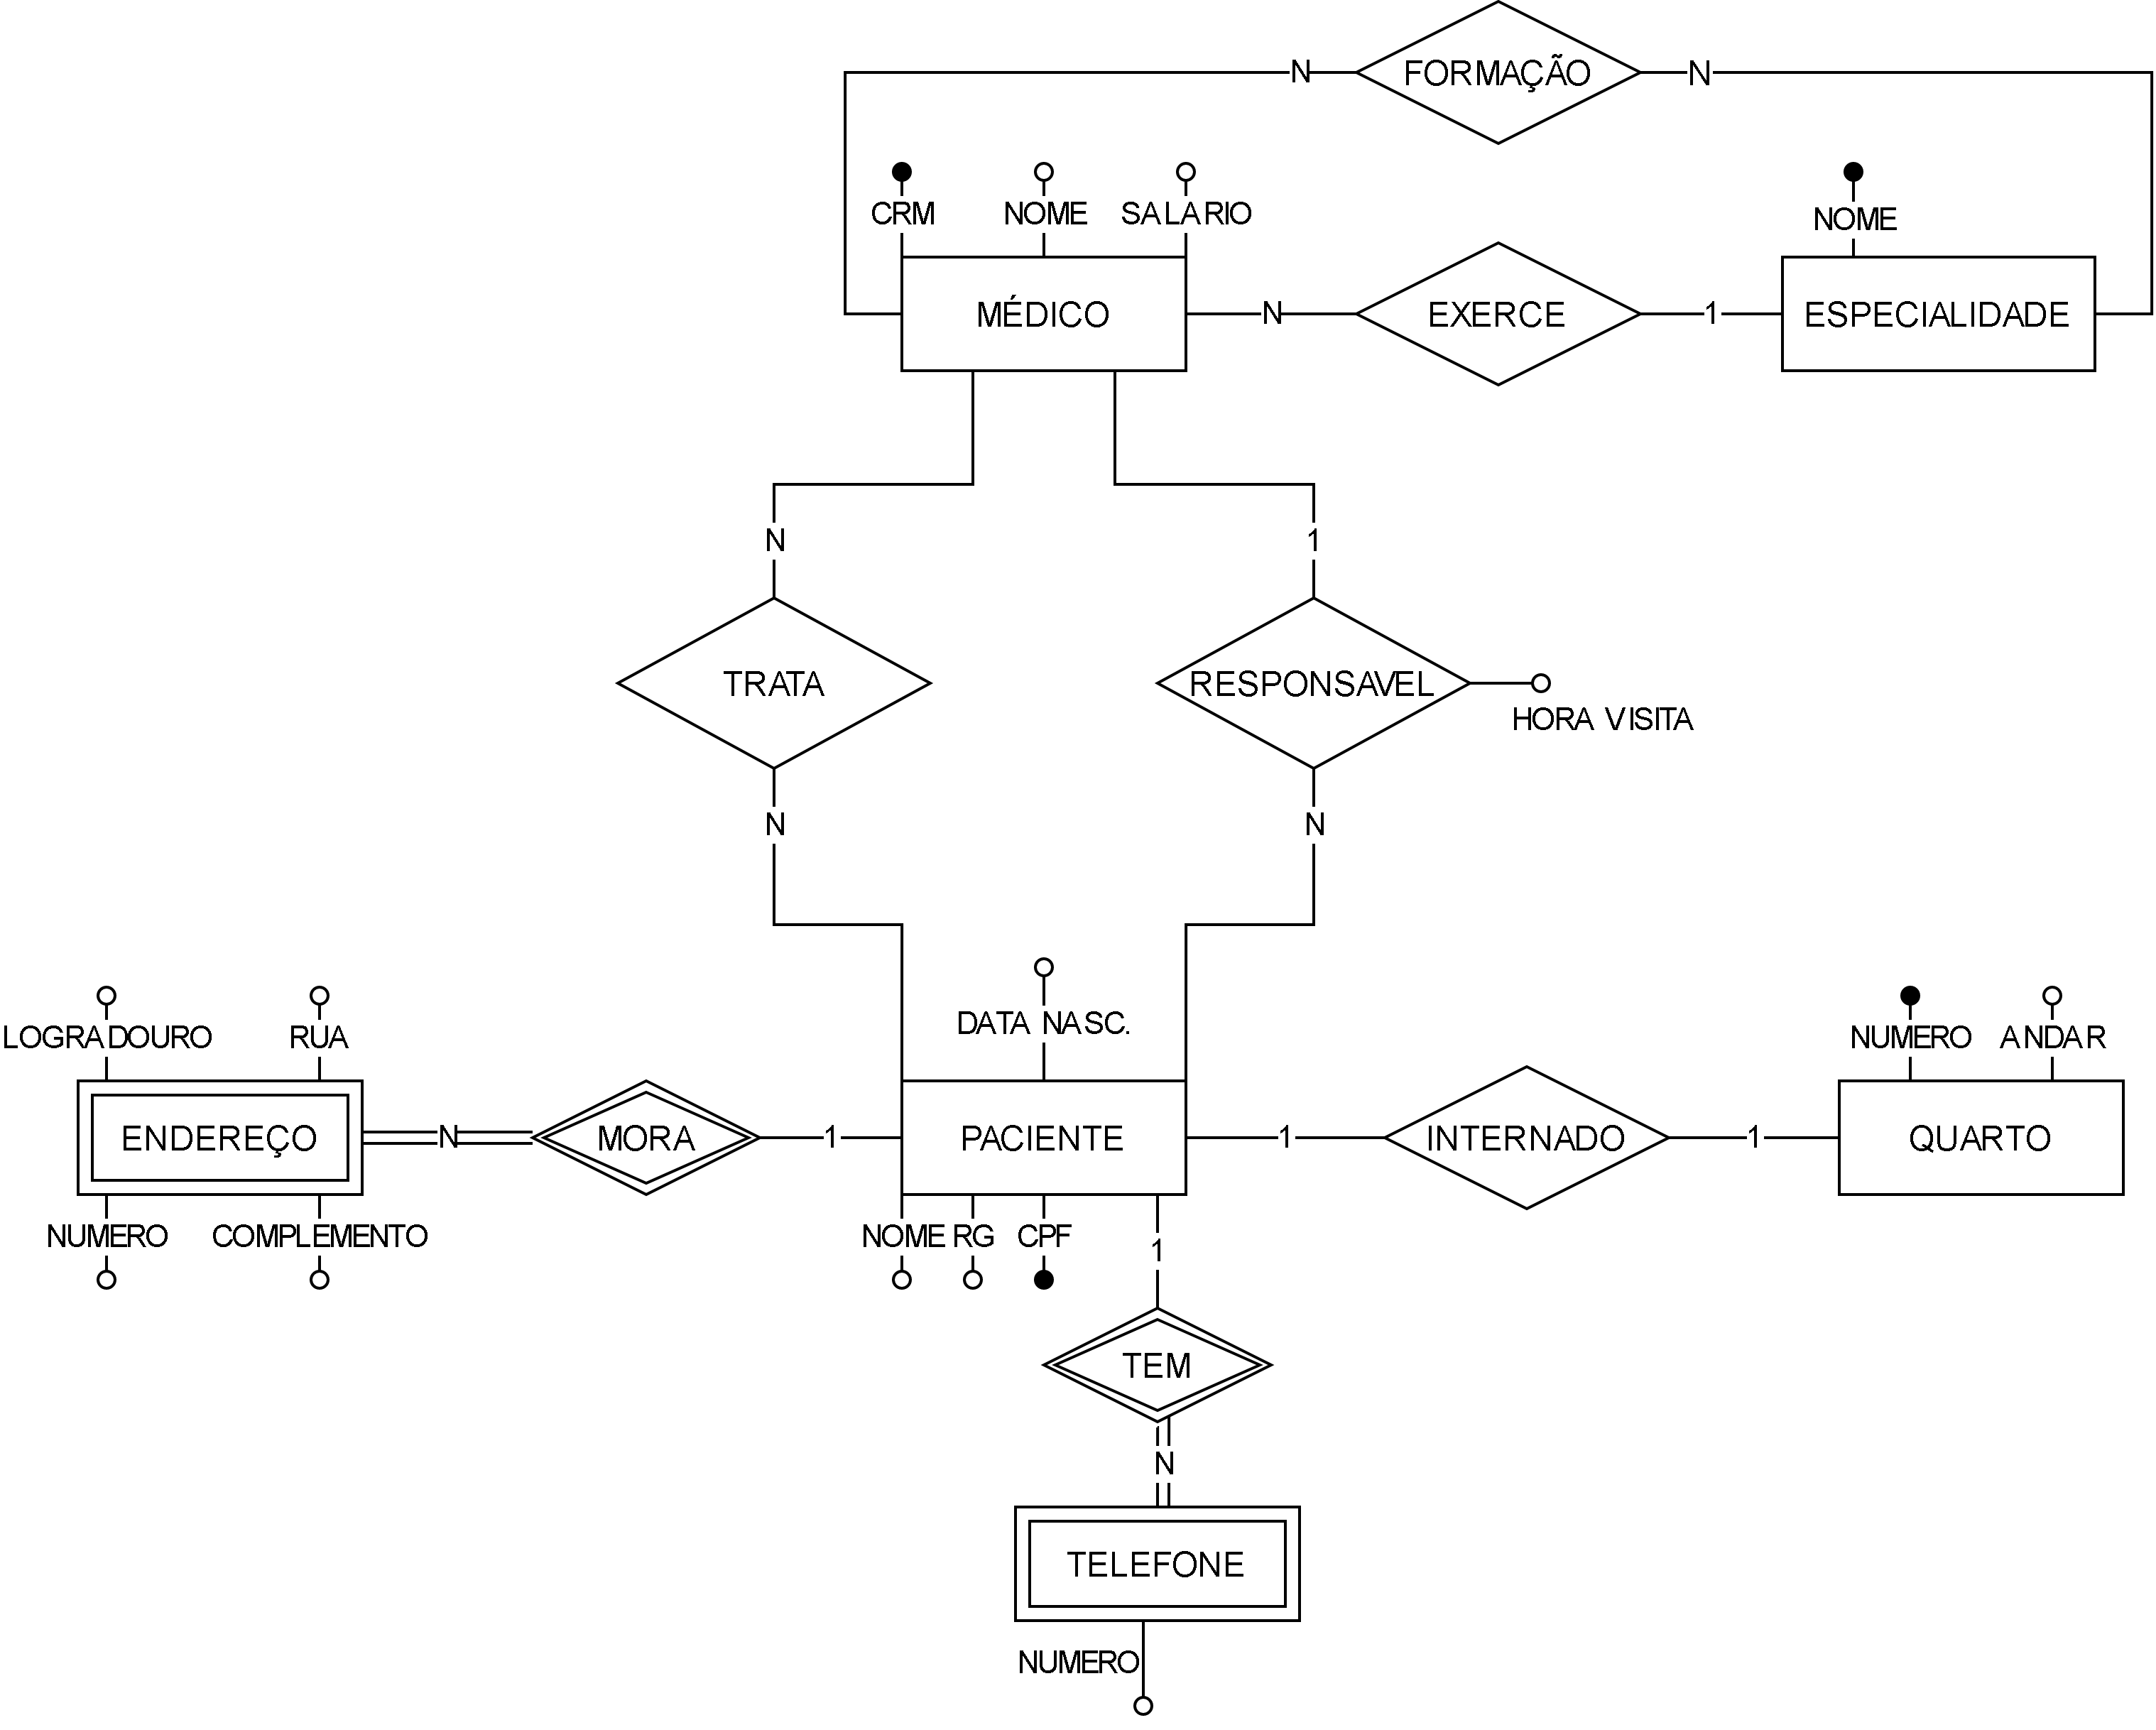
\includegraphics[width=1\textwidth]{LISTA 01 - EX 2 RESOLUÇÃO.png}
		\end{figure}
		\newpage
		
		\item \textbf{Locadora:} Uma pequena locadora de vídeos possui ao redor de 2000 DVDs, cujo empréstimo deve ser
		controlado. Cada DVD possui um número de identificação e contém um único filme. Cada filme
		recebe um identificador próprio, e sabe-se título e categoria (comédia, drama, aventura,...).
		
		Para cada filme cadastrado há pelo menos um DVD. Além disso, filmes mais longos necessitam de dois DVDs. Os clientes podem desejar encontrar os filmes estrelados pelo seu ator
		predileto. Por isso, é necessário manter a informação dos atores que estrelam em cada filme,
		mas nem todo filme possui estrelas. Muitos clientes, quando vêem a listagem de atores do
		filme escolhido, ficam interessados em saber, para um determinado ator, o seu nome real e de
		quais outros filmes do mesmo gênero aquele ator participou. A locadora possui muitos clientes
		cadastrados, dos quais sabe-se nome e sobrenome, telefone e seu endereço de contato. Além
		disso, cada cliente recebe um número de associado. Finalmente, o sistema deve permitir a
		consulta a empréstimos de DVDs, com informações de qual cliente alugou o quê, datas de
		empréstimo e devolução, valor pago ou a pagar, atrasos, etc... Não são mantidos registros
		históricos de empréstimos.
		
		\begin{figure}[H]
			\centering
			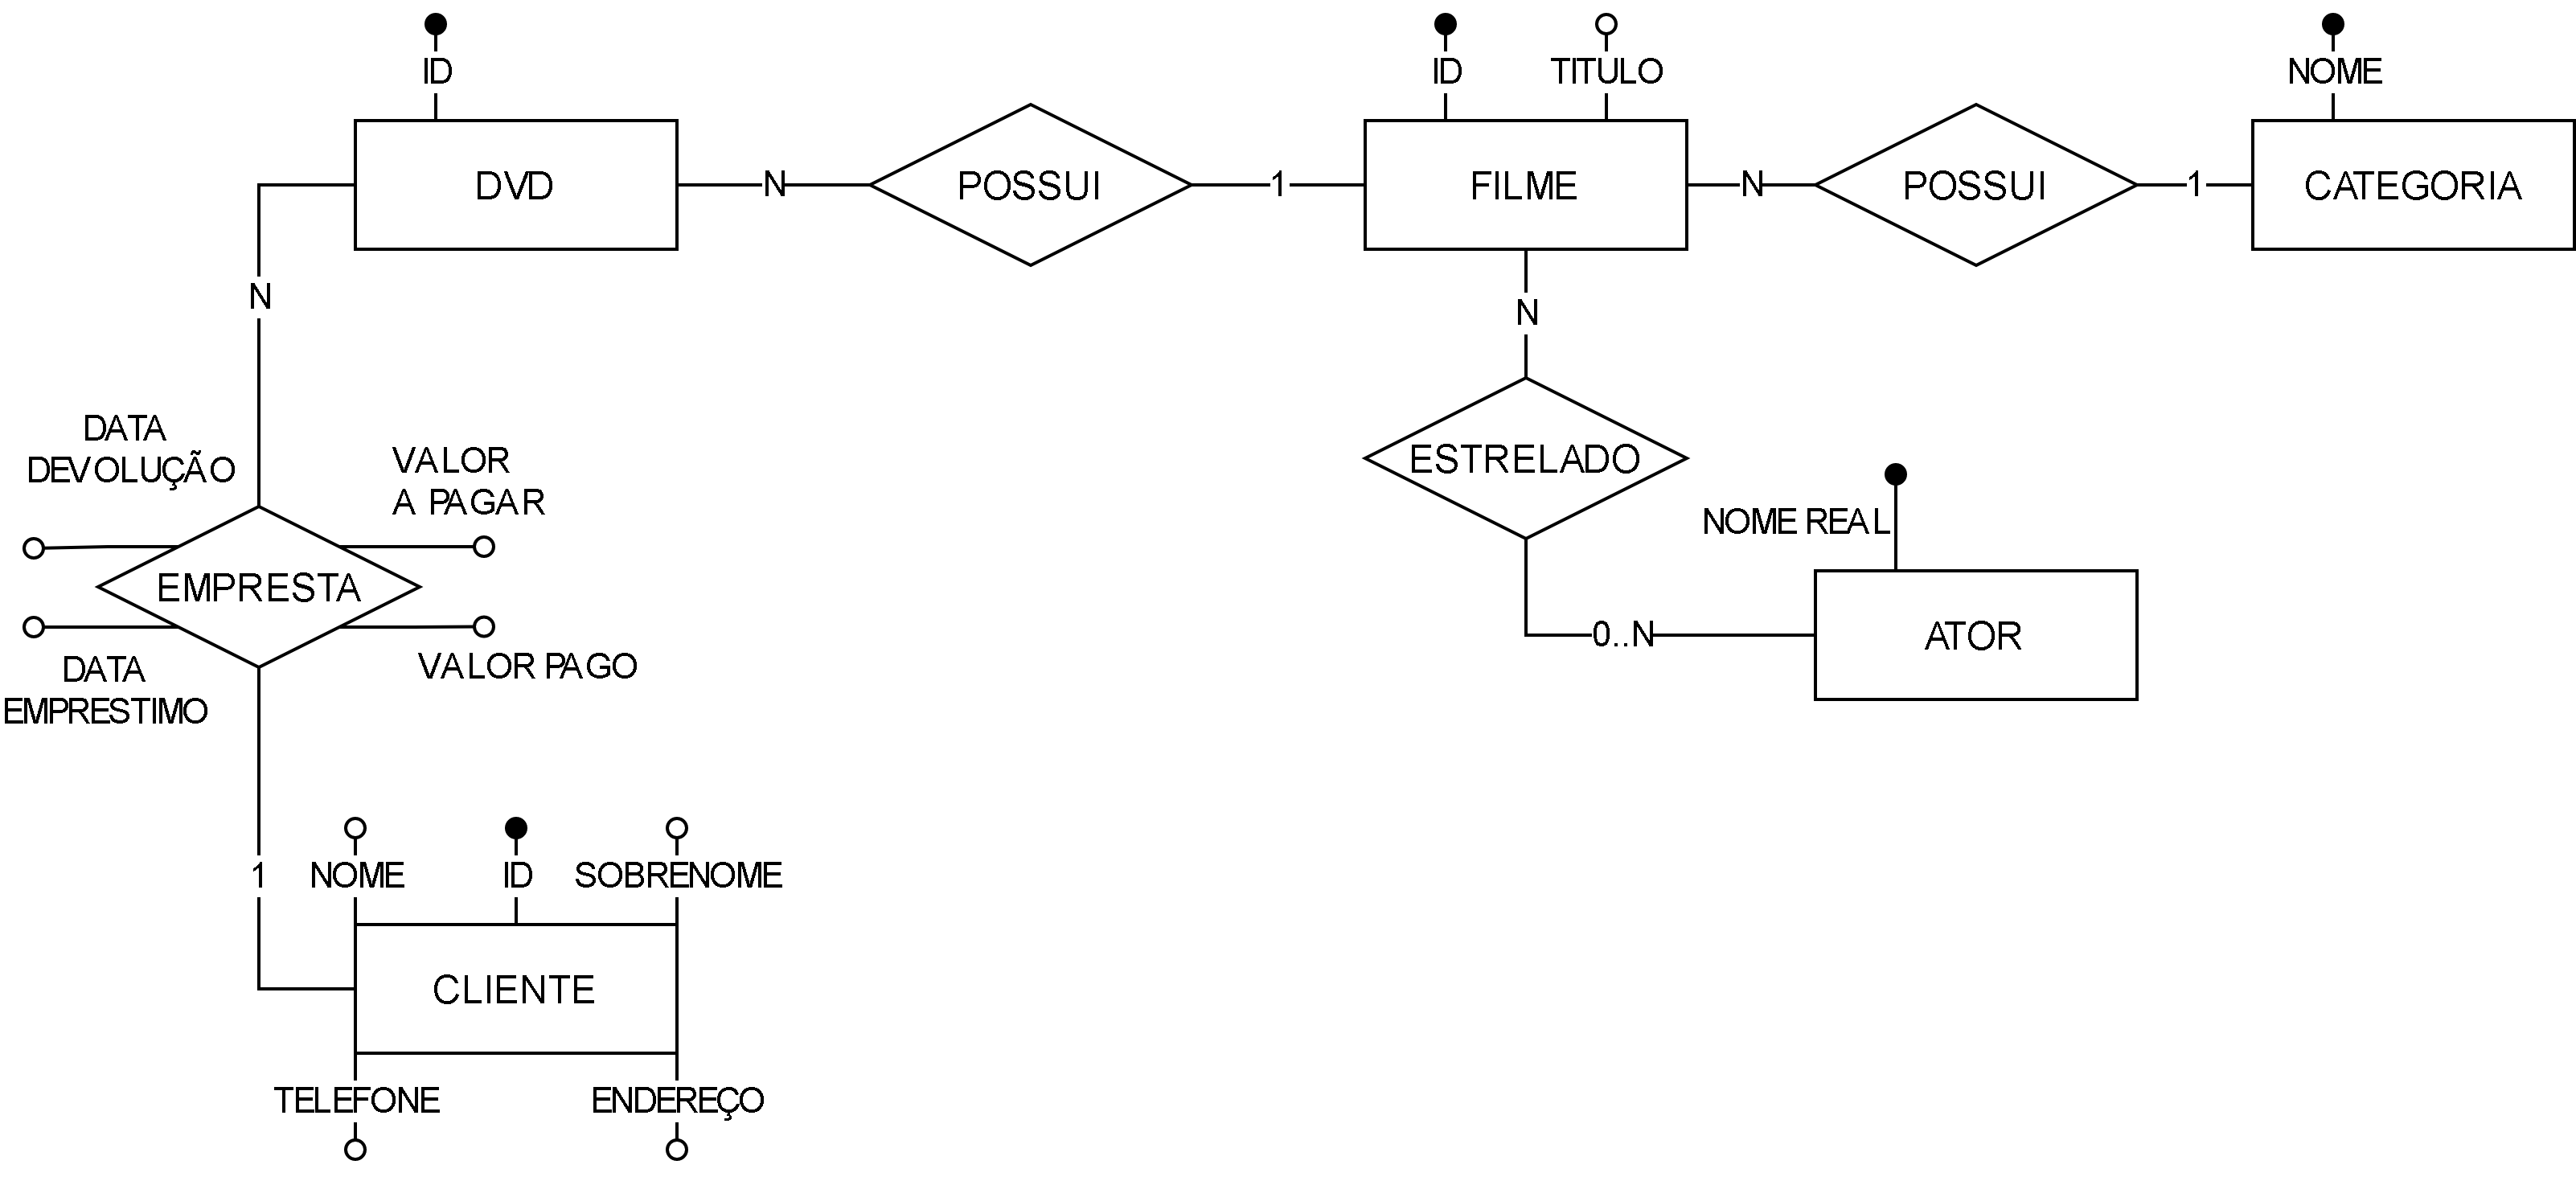
\includegraphics[width=1\textwidth]{LISTA 01 - EX 3 RESOLUÇÃO.png}
		\end{figure}
		\newpage
		
		\item \textbf{Oficina Mecânica:} Uma empresa de reparo de automóveis pretende implementar um sistema para administrar a
		informação relativa aos reparos efetuados nos veículos de seus clientes. O sistema de informação deverá permitir manter um registro de todos os reparos efetuados. A empresa registra
		as seguintes informações de cada cliente: código de identificação, nome, endereço, telefone.
		A informação relativa aos veículos que um dado cliente teve ou tem e as datas em que fizeram o primeiro reparo, também são importantes. Em relação aos funcionários da oficina é
		necessário registrar a seguinte informação: código de identificação, nome, endereço, telefone
		e categoria profissional. O custo/hora da mão-de-obra depende da categoria do funcionário e
		é definido por meio de uma tabela que é atualizada regularmente. Em relação a cada reparo
		é necessário saber: qual veículo, qual cliente, a data em que o reparo foi efetuado e o custo
		total do reparo. A empresa pretende saber para cada reparo quais peças foram utilizadas e o
		seu preço, bem como o tempo de mão de obra gasto por cada funcionário e o respectivo custo.
		A informação relativa às peças em estoque deverá ser: código de identificação, designação,
		custo unitário e quantidade armazenada.
		
		\begin{figure}[H]
			\centering
			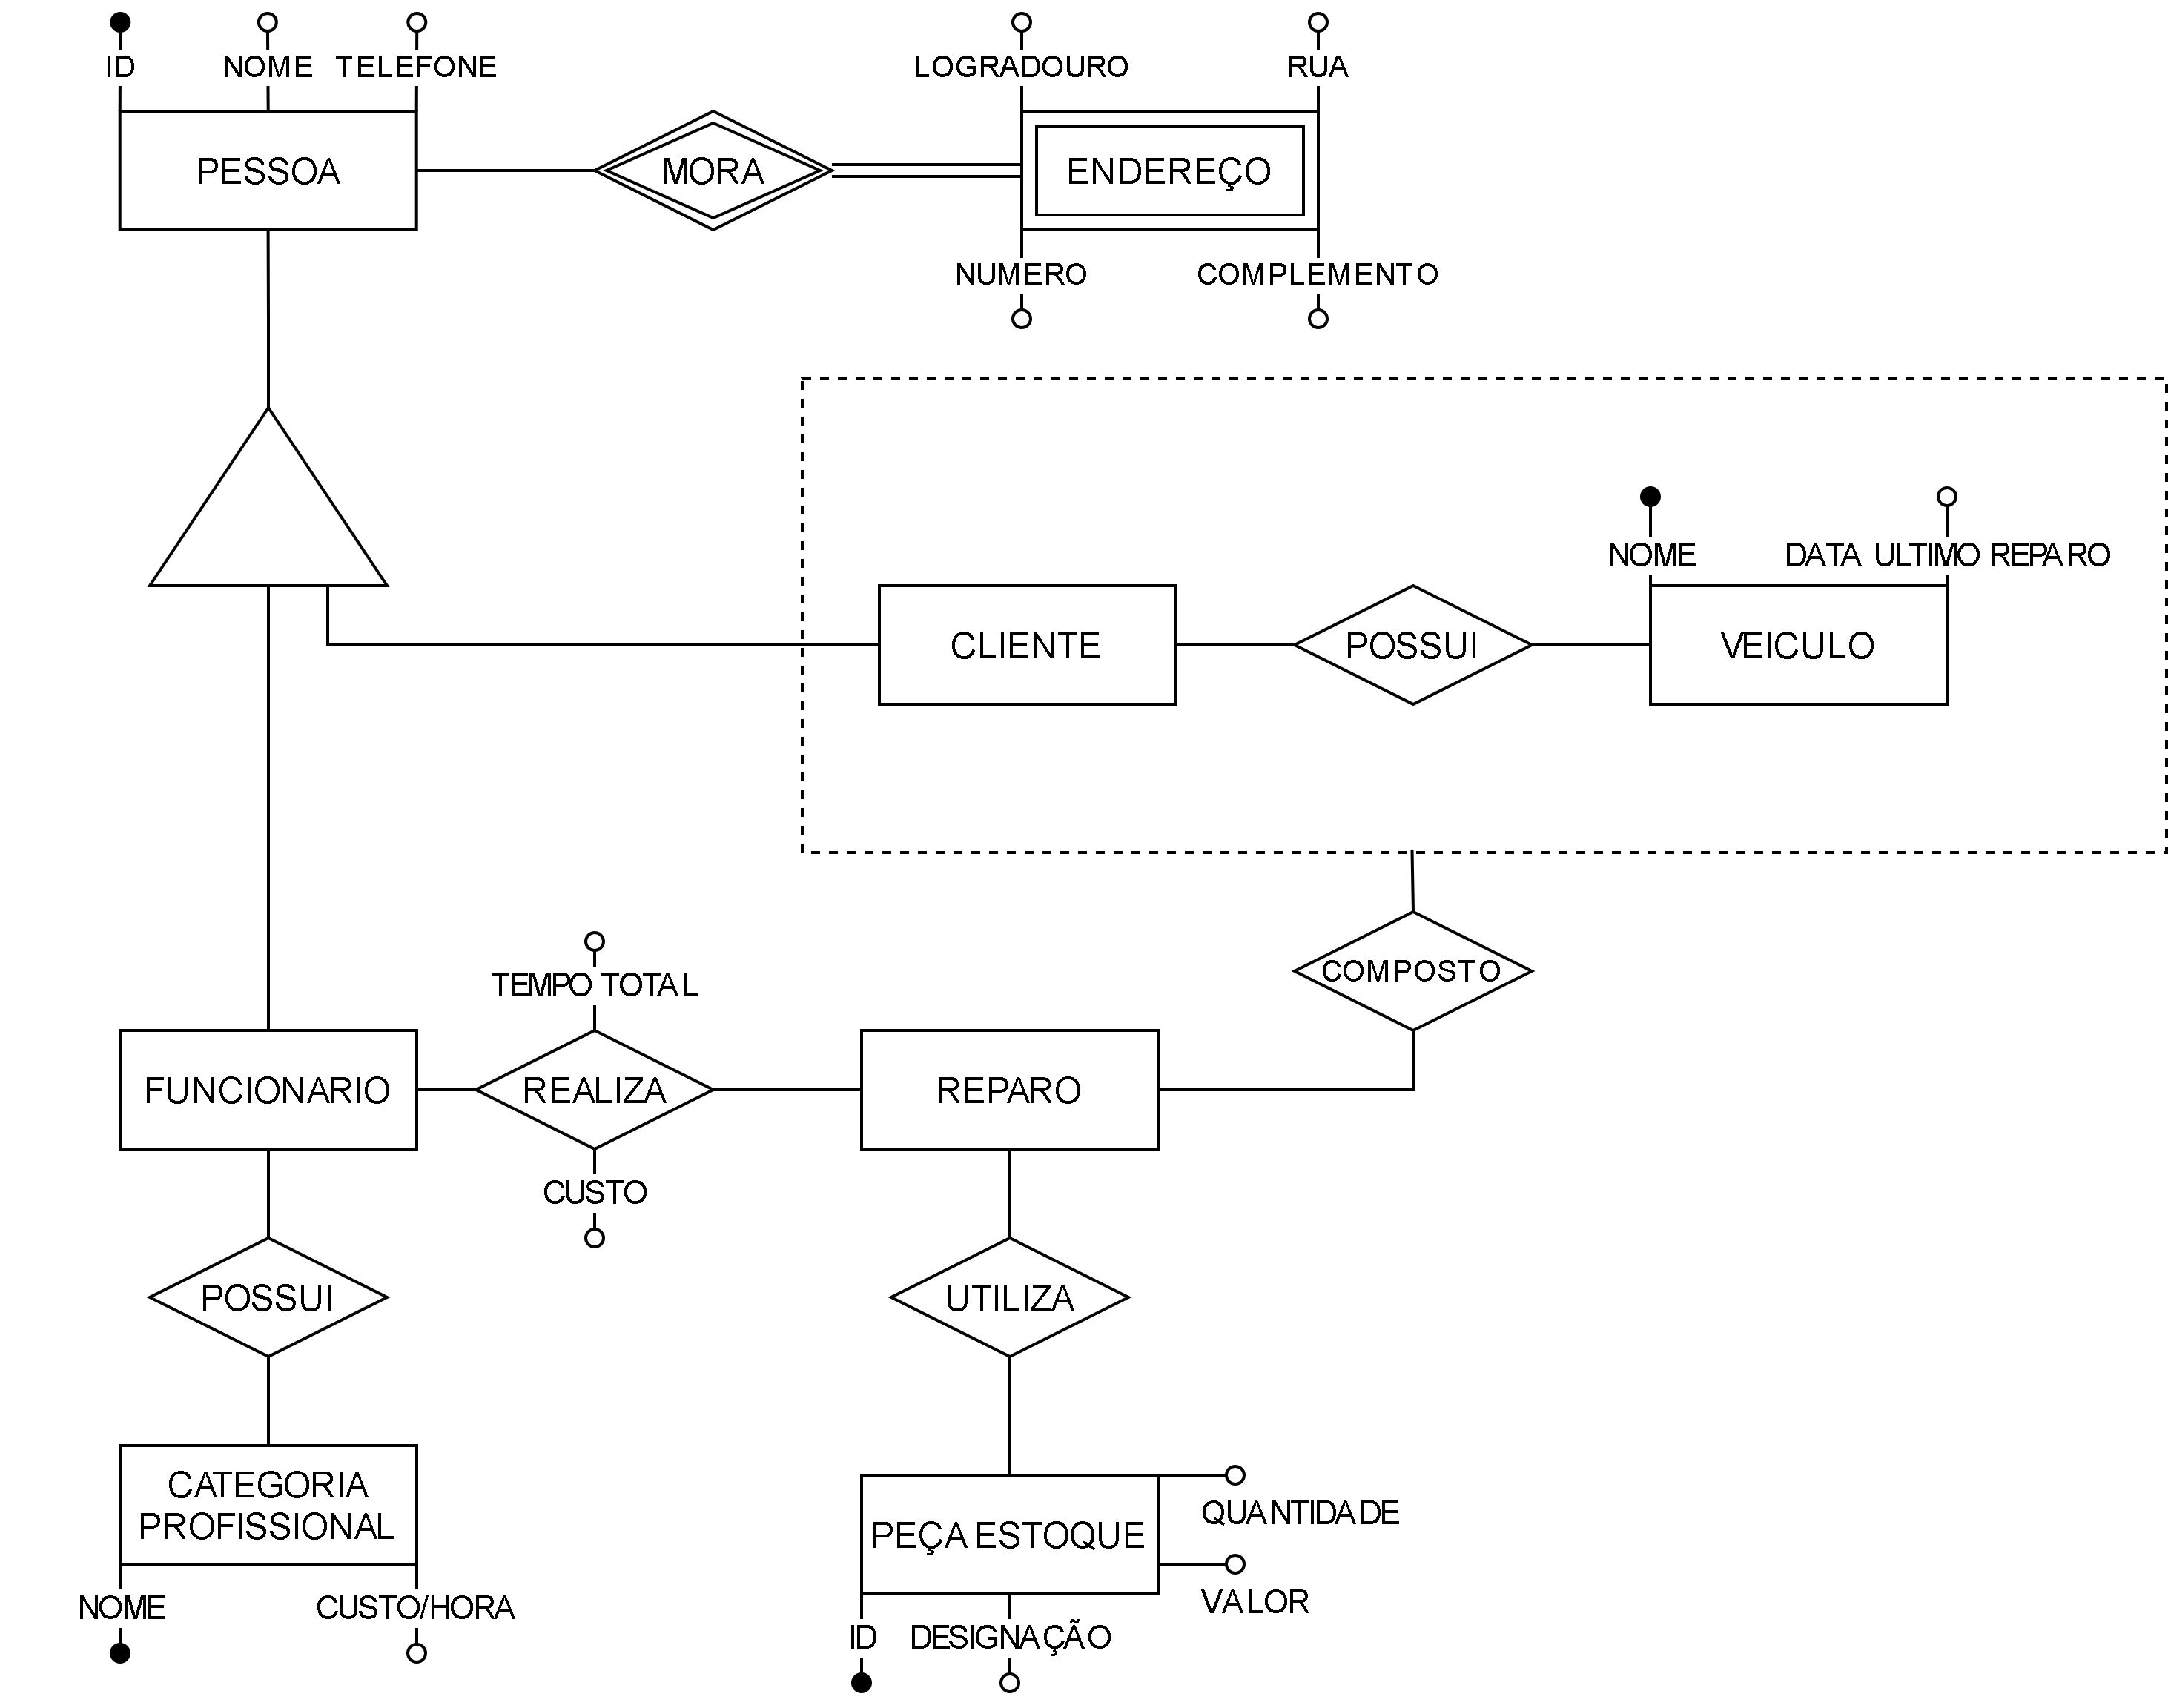
\includegraphics[width=1\textwidth]{LISTA 01 - EX 4 RESOLUÇÃO.png}
		\end{figure}
		\newpage
		
		\item \textbf{Faculdade:} Uma faculdade oferece vários cursos cujos currículos são compostos por diversas disciplinas.
		Cada disciplina pode ser oferecida para vários cursos distintos; uma disciplina pode ter outras
		disciplinas como pré-requisitos em série ou em paralelo. Na faculdade há diferentes tipos de
		pessoas identificadas por um único número funcional: os alunos, professores e funcionários –
		cada qual com seus atributos gerais e específicos (defina alguns). Os alunos como na USP, só
		podem estar inscritos em um único curso em um dado momento (status ativo), e só poderão se
		inscrever em outro curso caso todas as suas inscrições estejam finalizadas (status concluído)
		– são armazenadas informações de ano de início e de término. Em cada semestre, os alunos matriculam-se em turmas correspondentes às disciplinas do seu curso. Professores podem
		ministrar para várias turmas, e toda turma tem obrigatoriamente um professor. Os funcionários
		auxiliam os professores, sem exclusividade. Tanto os professores quanto os funcionários podem decidir se matricular em um curso da universidade, com as devidas restrições. A base de
		dados deve permitir a geração de listas de notas para cada turma, onde deve constar com que
		professor um aluno fez qual disciplina.  
		
		\begin{figure}[H]
			\centering
			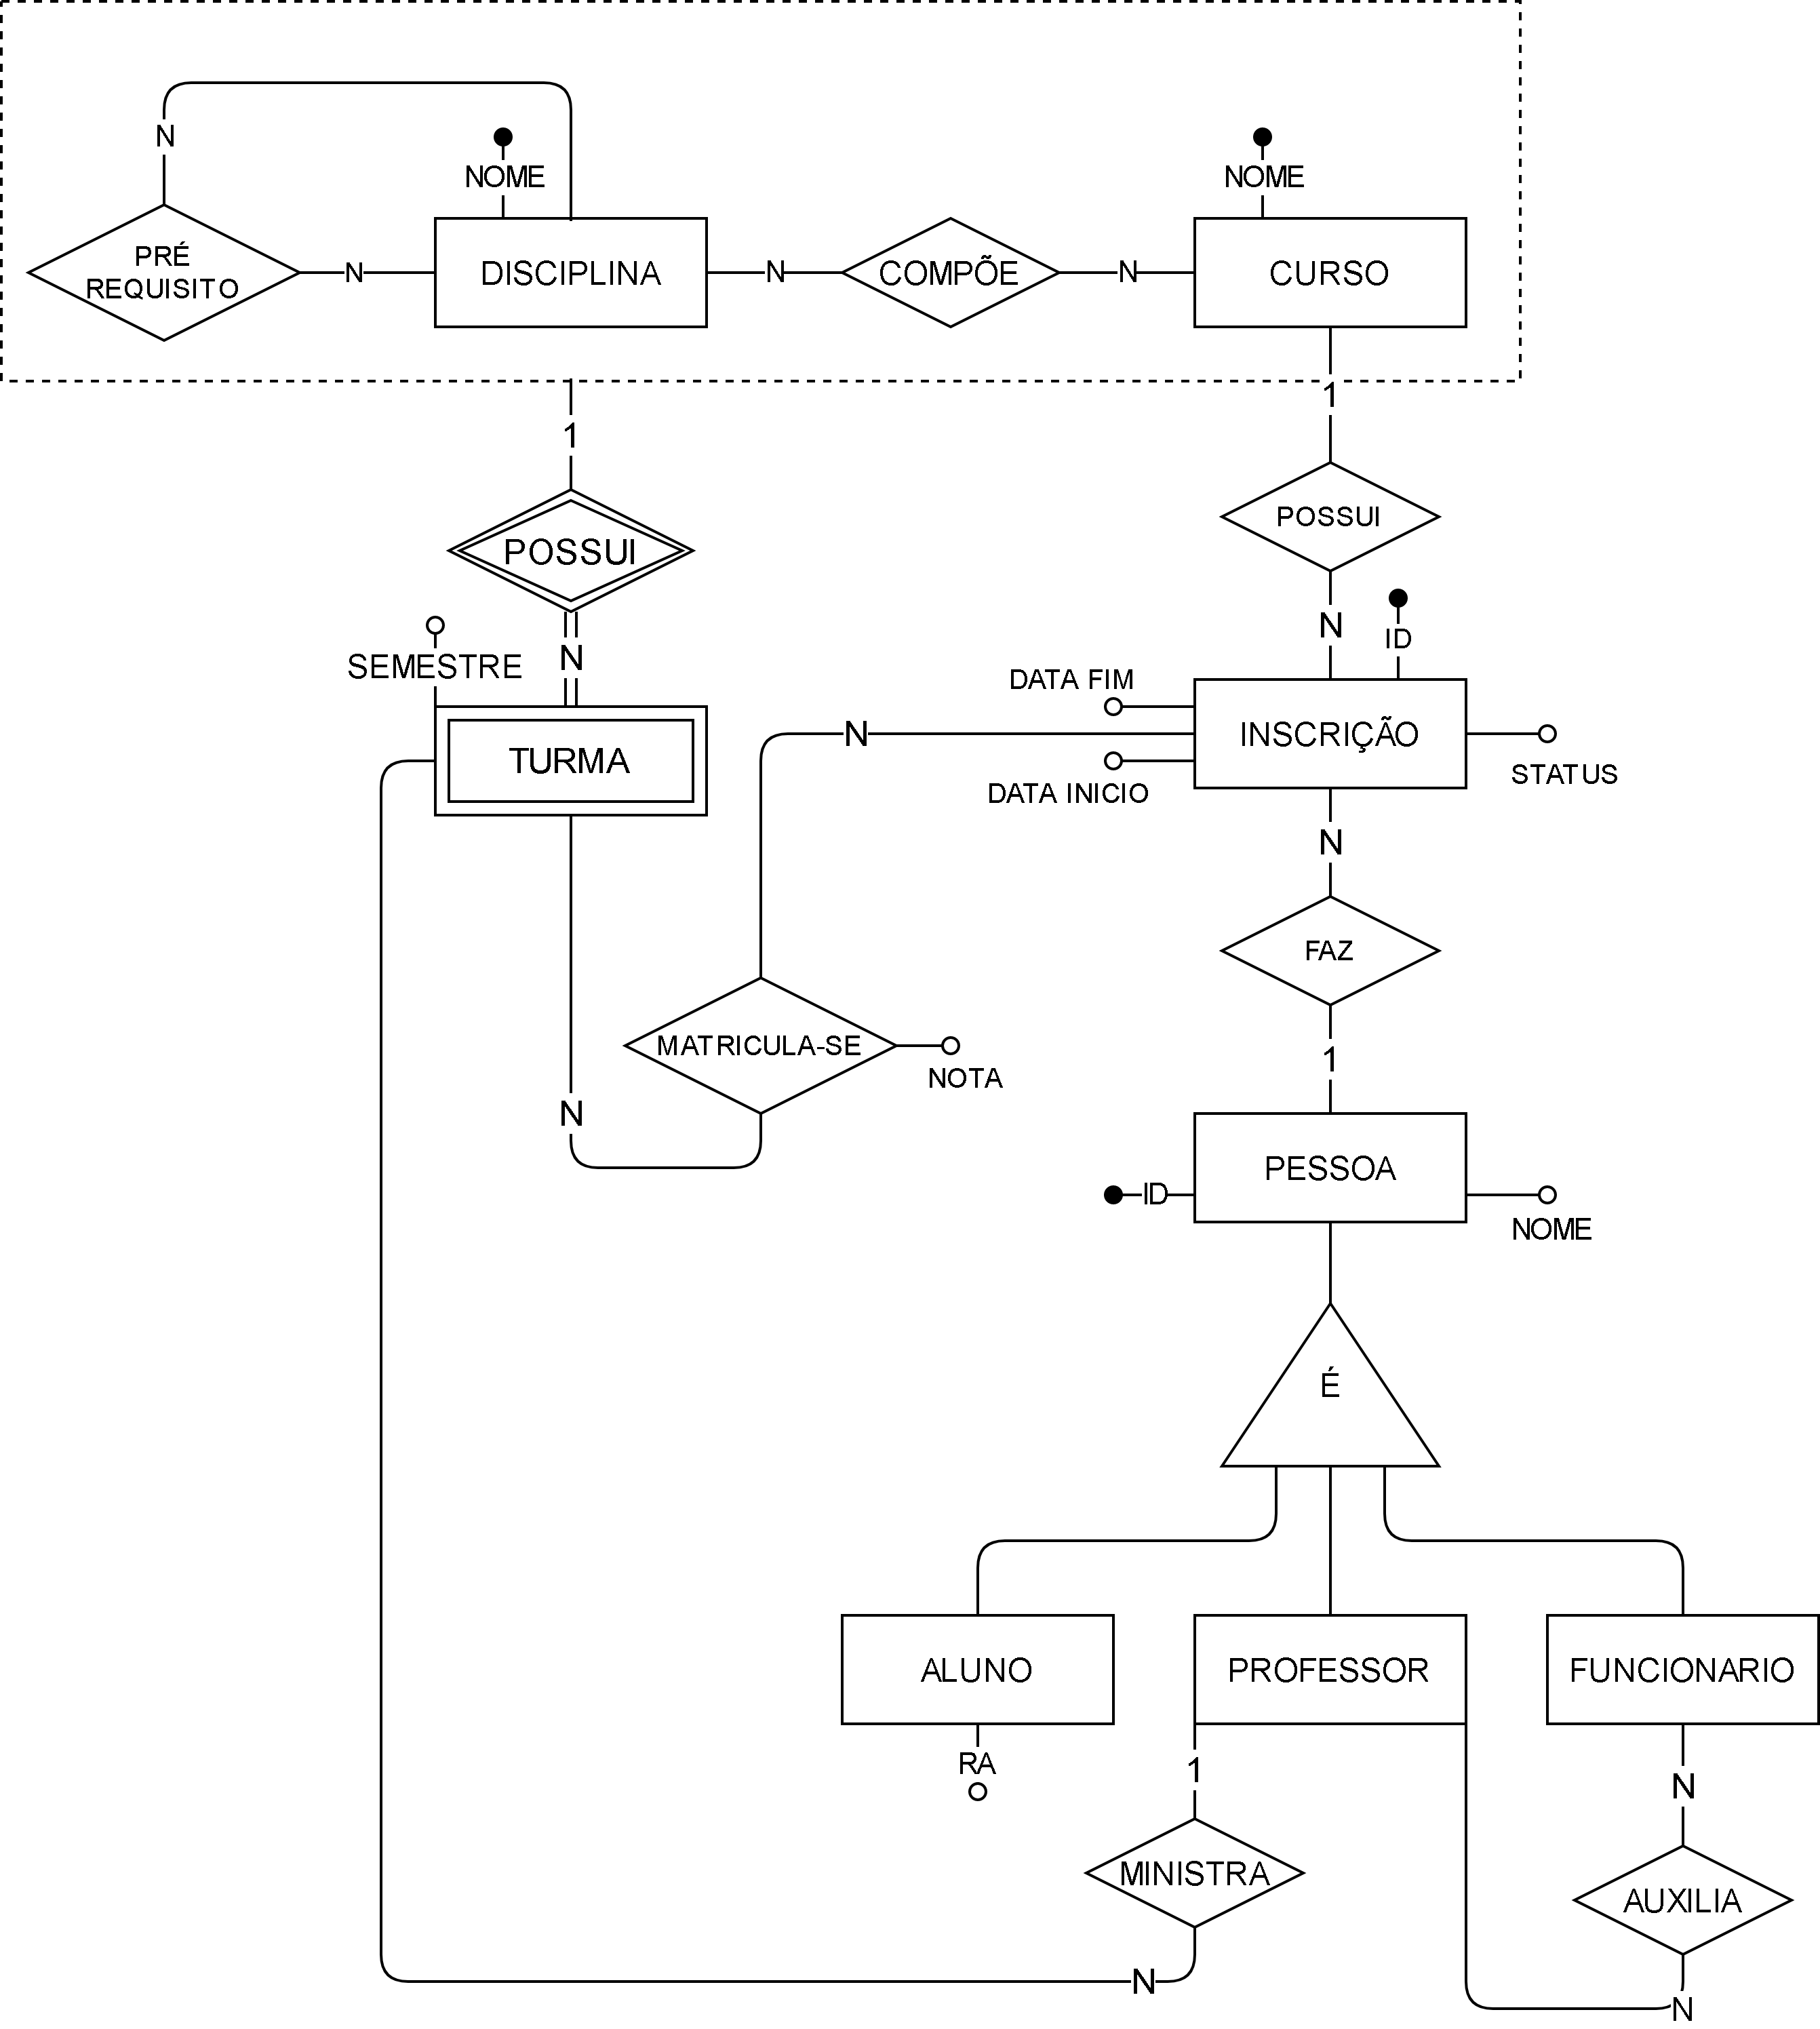
\includegraphics[width=0.7\textwidth]{LISTA 01 - EX 5 RESOLUÇÃO.png}
		\end{figure}
		\newpage
		
		\item \textbf{Picolés:} Uma empresa fabricante de picolés deseja armazenar informações acerca de seus negócios.
		Os picolés fabricados são divididos em normal (com água) e ao leite. As informações comuns
		armazenadas dos picolés são: sabor, ingredientes, preço e tipo da embalagem. Especificamente, picolés normais possuem um conjunto de aditivos nutritivos (vitaminas ou sais minerais)
		cada um com nome e fórmula química; e picolés ao leite contêm um conjunto de conservantes
		cada um com nome e descrição. Os dois tipos de picolé são vendidos em lotes exclusivos (ou
		normais ou ao leite) para os revendedores, e cada lote gera um conjunto de notas fiscais com
		data, valor, número de série e descrição. Todo revendedor possui uma pessoa de contato para
		eventuais resoluções de problemas, além disso, armazenam-se do revendedor CNPJ e razão
		social. Deseja-se obter relatórios sobre as vendas mensais dos picolés de cata tipo e quais
		revendedores compraram mais picolés nos últimos meses.
		
		\begin{figure}[H]
			\centering
			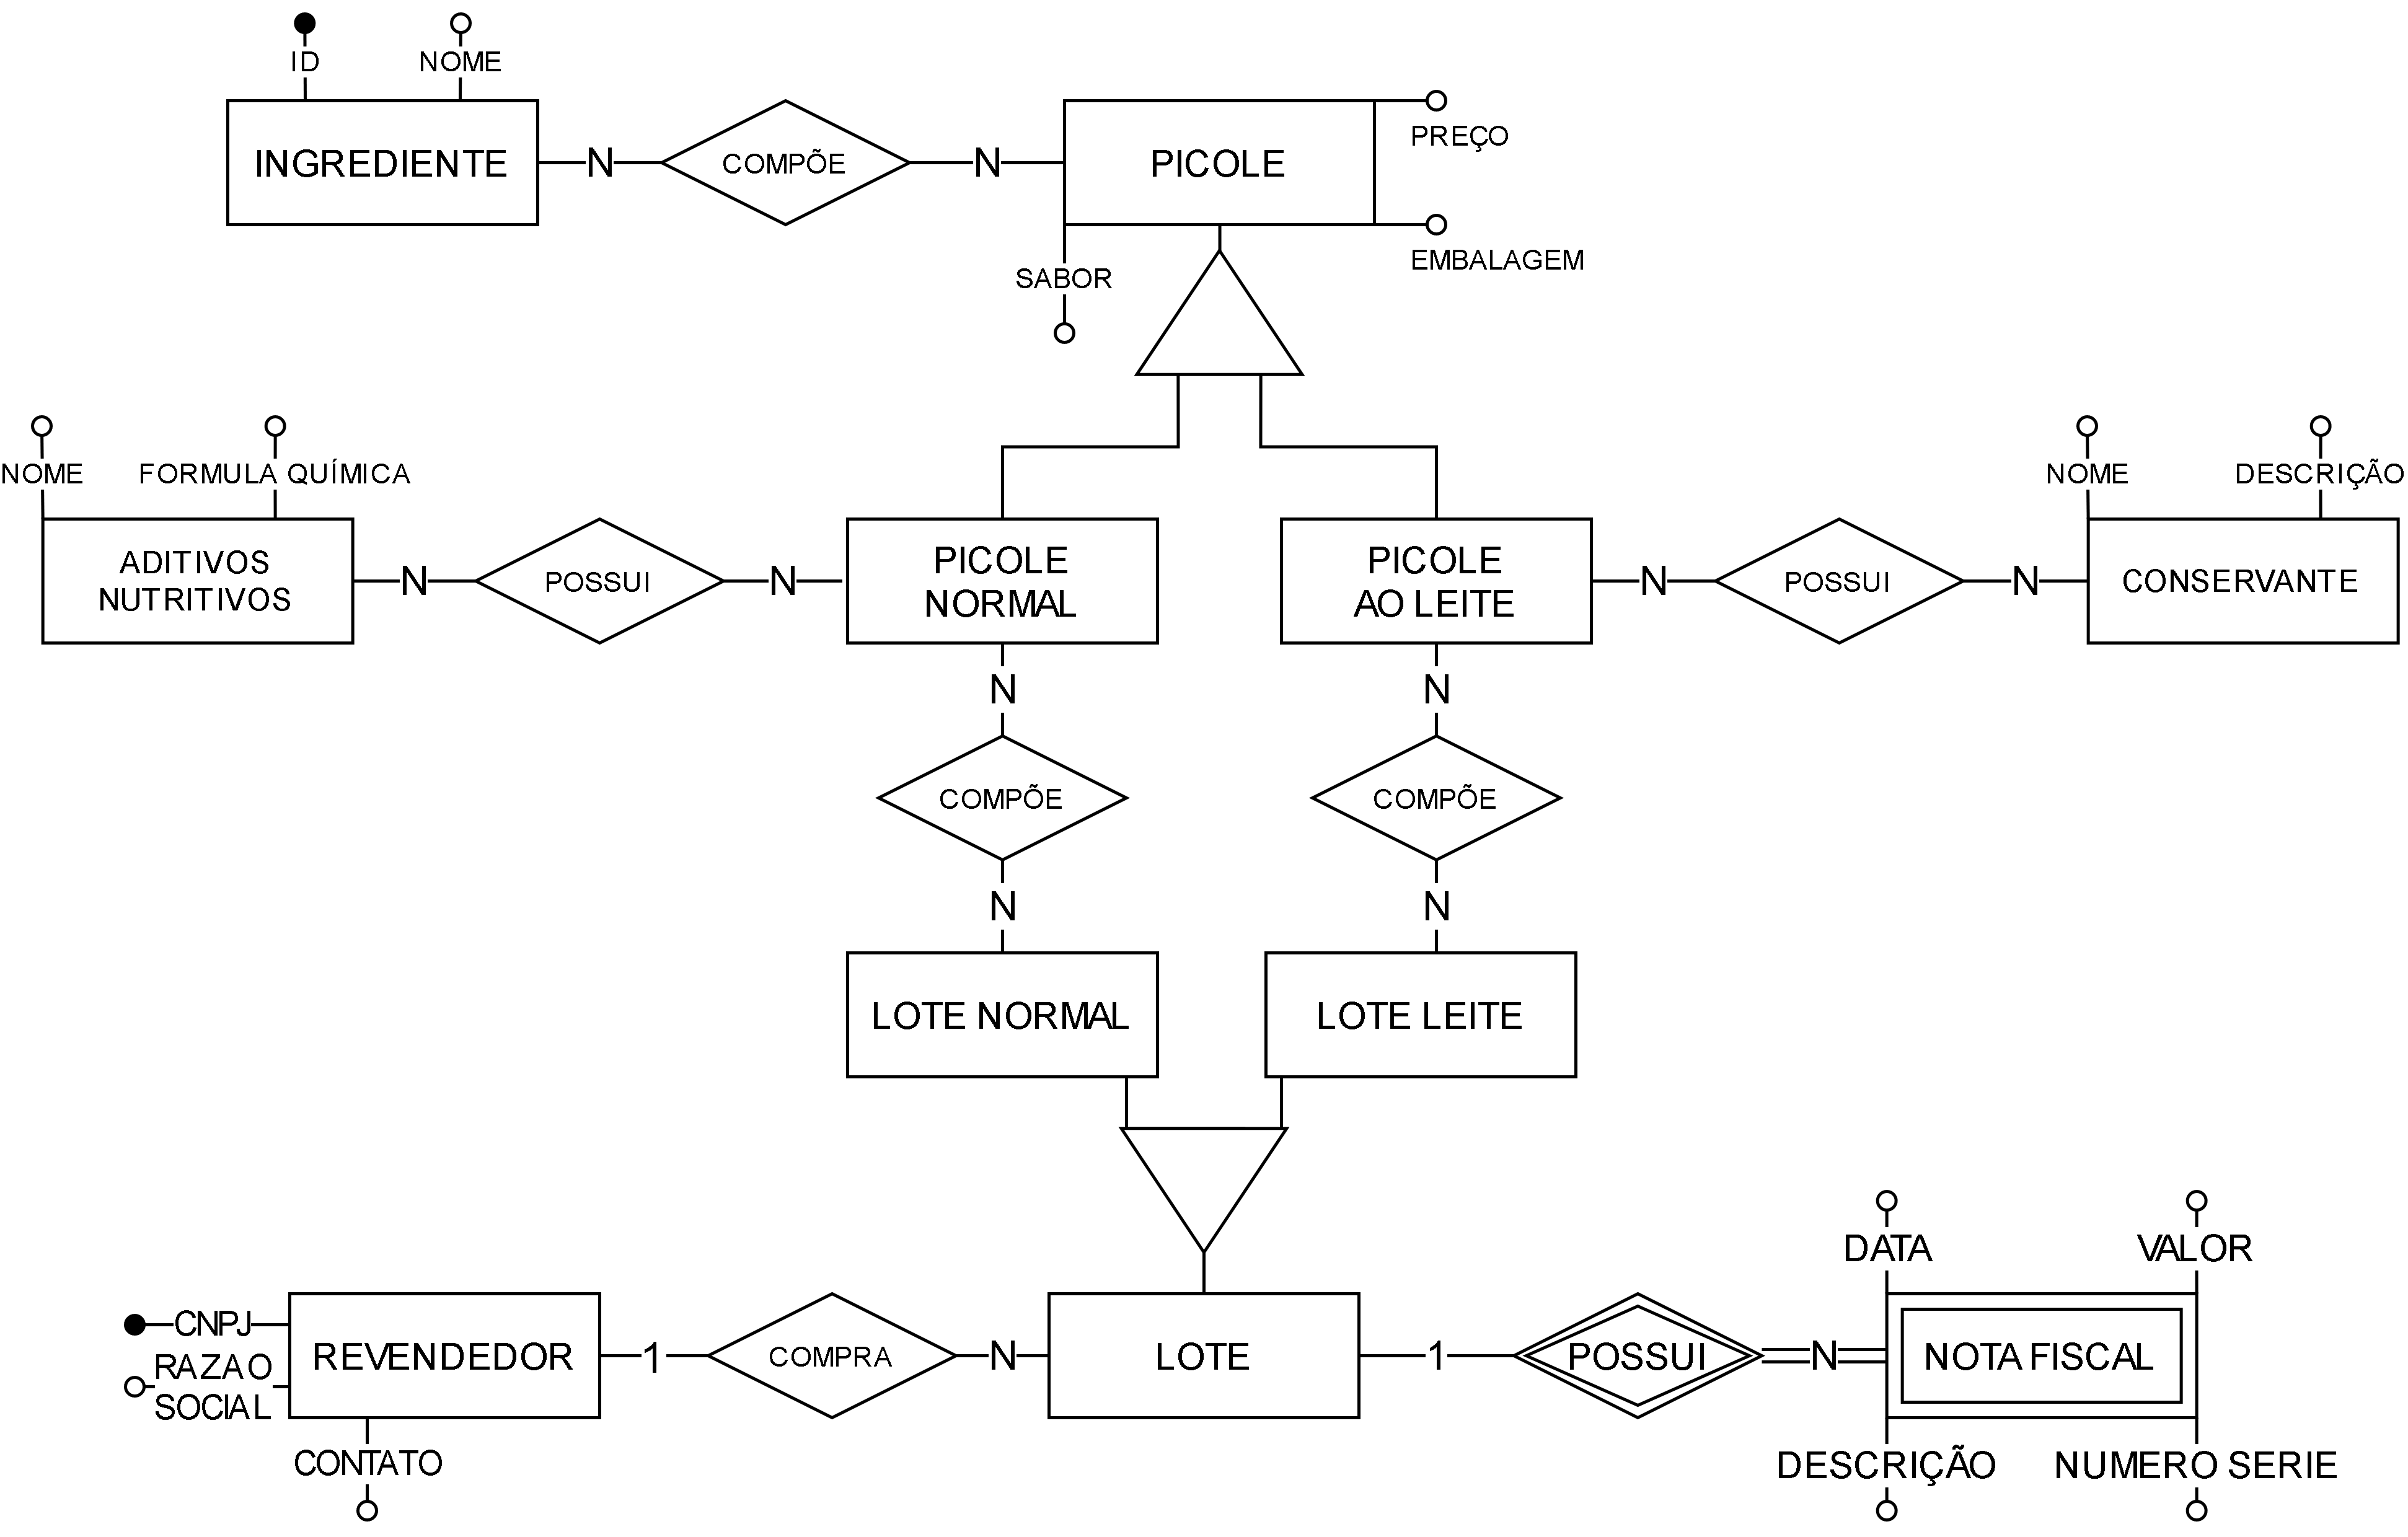
\includegraphics[width=1\textwidth]{LISTA 01 - EX 6 RESOLUÇÃO.png}
		\end{figure}
		\newpage
		
		\item \textbf{Estacionamento:} Uma garagem para estacionamento de veículos pretende implementar um sistema que lhe
		permita administrar a informação relativa ao estacionamento dos seus clientes. A garagem é
		composta por um conjunto de vagas, cada uma podendo estar ocupada ou não. Há dois tipos
		de vagas: avulsa (se houver disponibilidade) ou mensal. Cada vaga tem um preço – a avulso
		tem um custo por hora e o mensal um custo fixo. Os preços serão diferenciados de acordo com
		o tipo de veículo: automóvel ou moto. Cada vaga mensal possui um cliente associado. Para
		cada cliente é registrado seu nome e CPF, sendo que um dado cliente pode contratar várias
		vagas mensais. A cada vez que um cliente estacionar um veículo (fizer uma “estacionagem”),
		deverá se armazenar o CPF do cliente, código da vaga, a data/hora de entrada e de saída, a
		placa do veículo estacionado e o custo gerado (que pode ser null para clientes mensais).
		
		\begin{figure}[H]
			\centering
			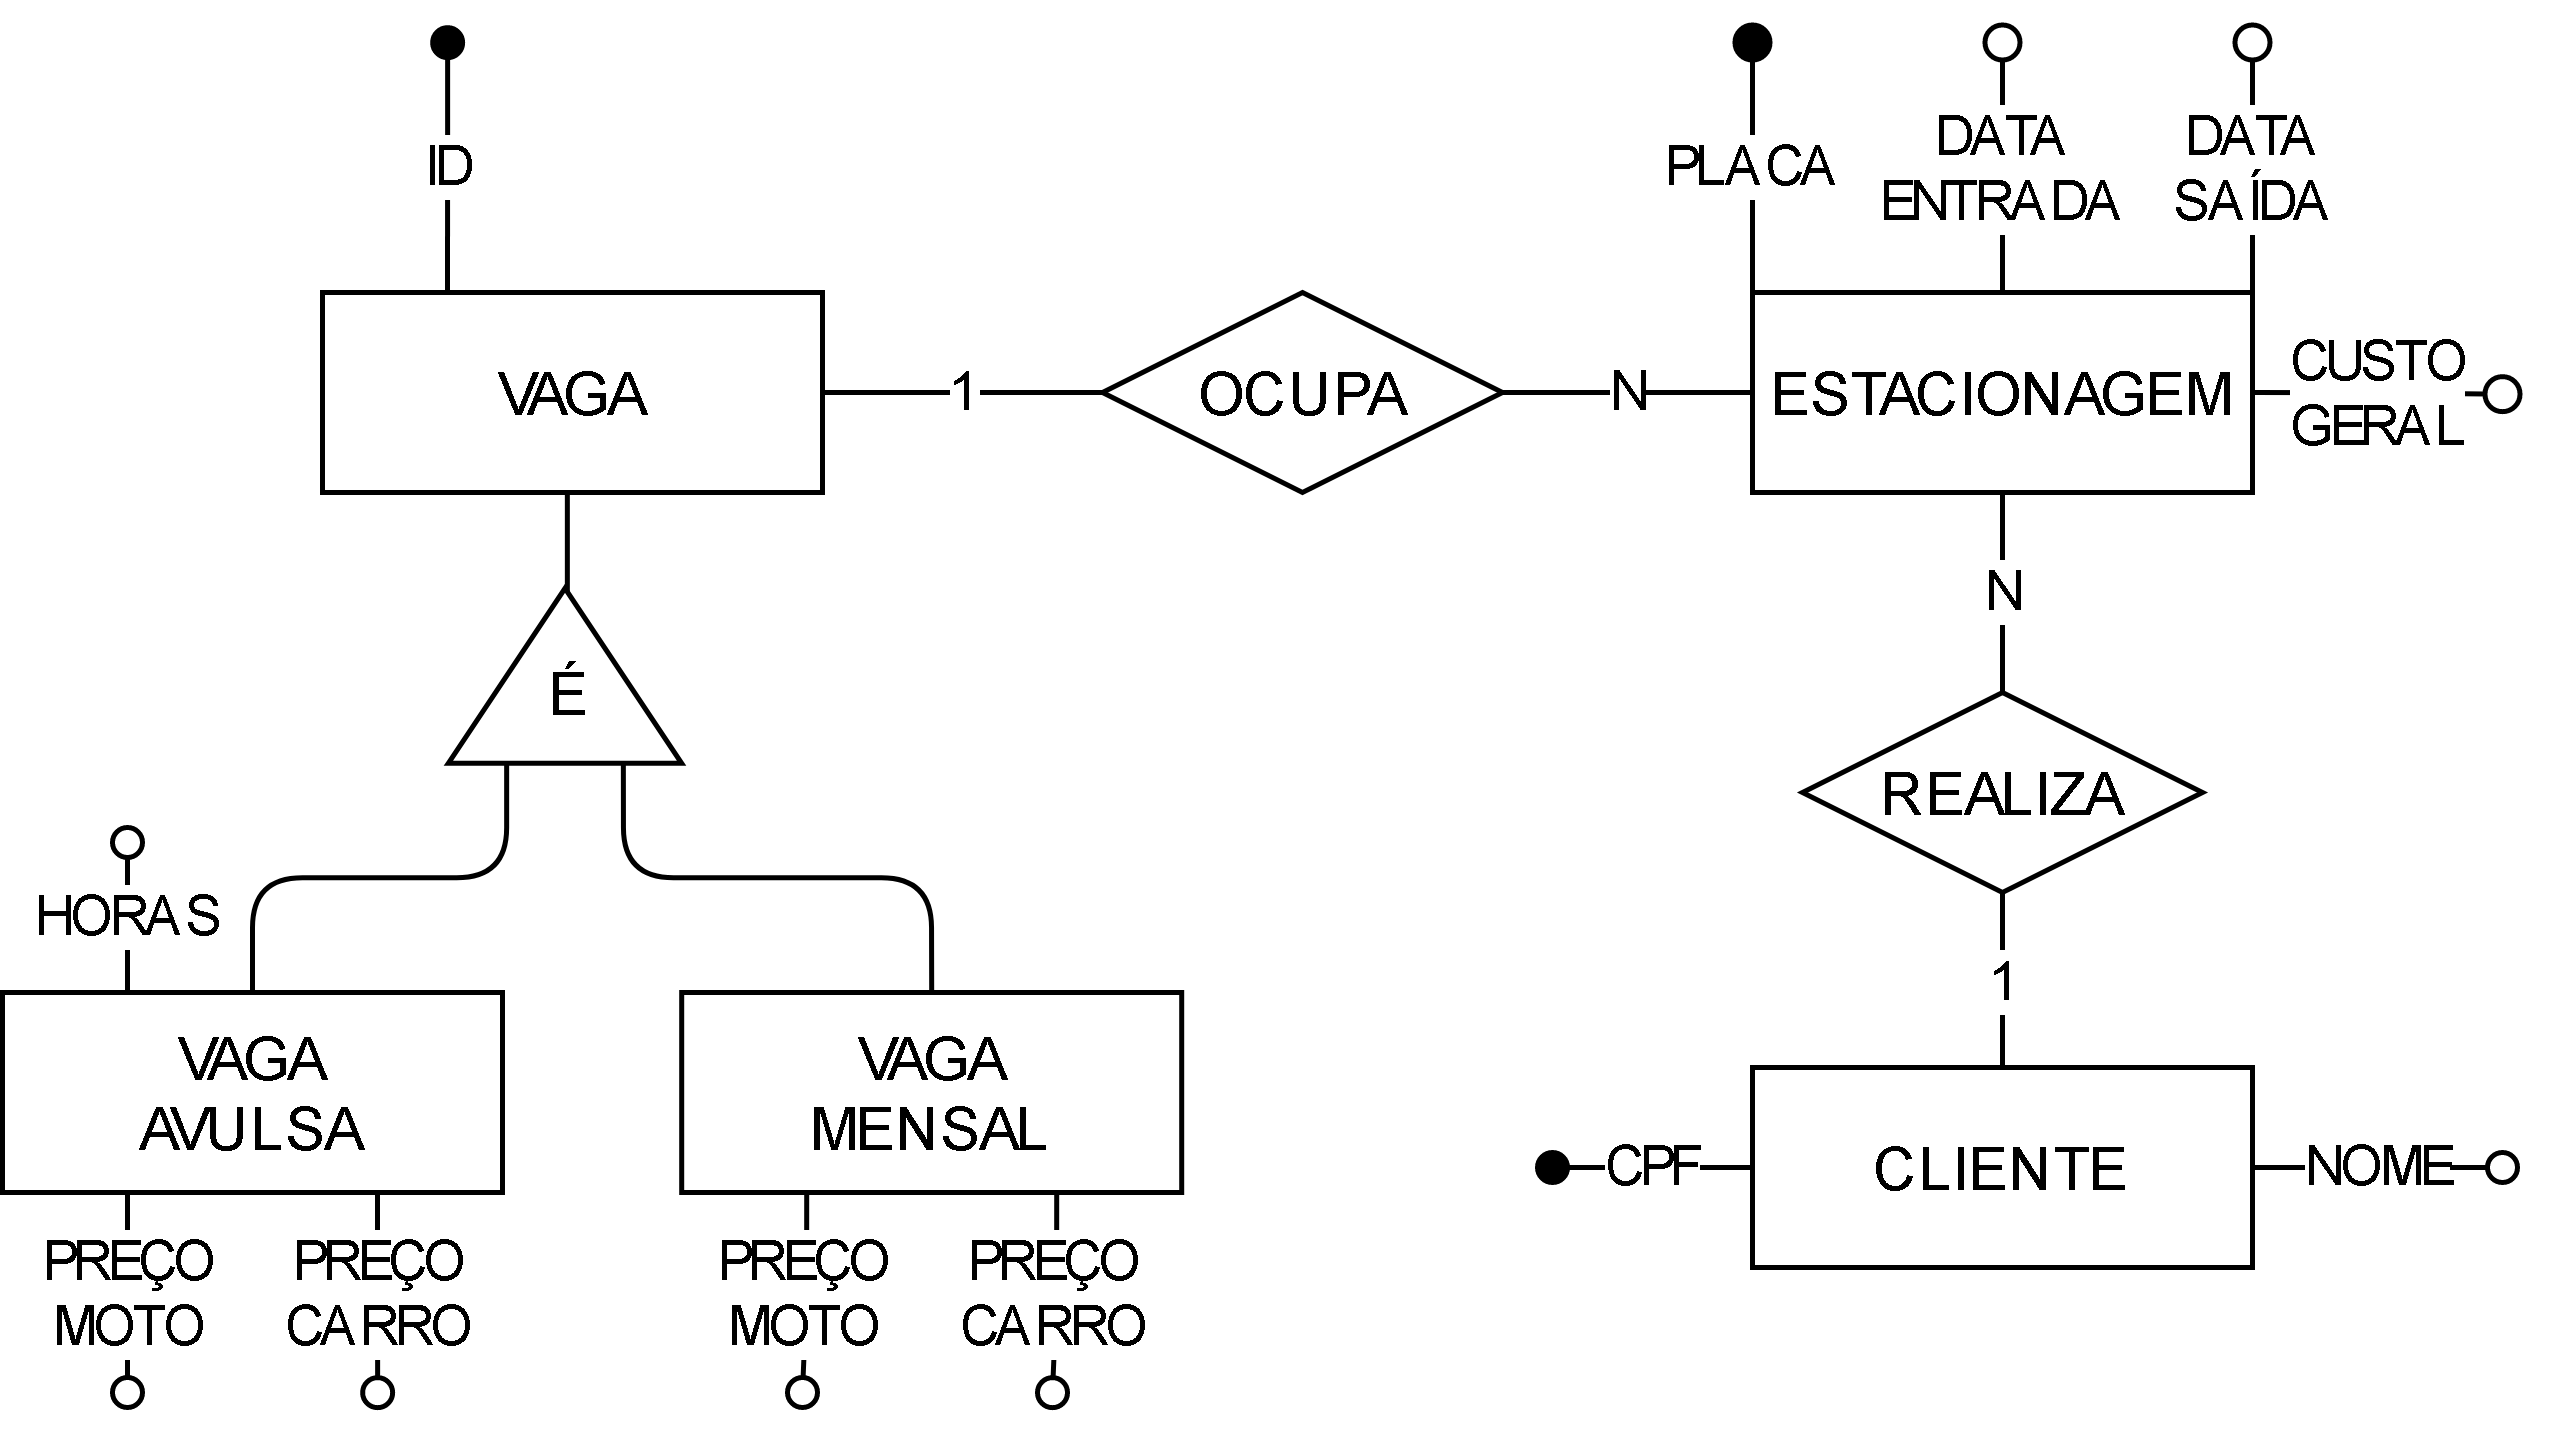
\includegraphics[width=1\textwidth]{LISTA 01 - EX 7 RESOLUÇÃO.png}
		\end{figure}
		\newpage
		
	\end{enumerate}
		
\end{document}
